%----------------------------------------------------------------------------------------
\chapter{MIT-Proto}
\label{chap:mitproto}
%----------------------------------------------------------------------------------------
In questo capitolo viene presentata la sintassi e i costrutti principali di Proto, al fine di fornire le basi necessarie per comprendere il \cref{chap:trasposizione}.
 
Per ulteriori dettagli sul linguaggio, si rimanda alla documentazione ufficiale\footnote{\url{https://github.com/jakebeal/MIT-Proto/blob/master/proto/man/proto-language-reference.pdf}}, da cui sono tratte le sezioni seguenti.

\section{Introduzione alla sintassi}
\label{sec:mitprotosyntax}


\paragraph{Valutazione delle espressioni}

Proto è un linguaggio puramente funzionale caratterizzato dall'utilizzo di \ac{sexp} (\Cref{lst:mitprotosexp}),  ovvero espressioni in notazione polacca racchiuse tra parentesi, adottando una sintassi molto simile a quella di Scheme\footnote{\url{https://www.scheme.org/}}.

\lstinputlisting[
    language=Lisp,
    label={lst:mitprotosexp},
    caption={Le espressioni in Proto sono scritte in notazione polacca, specificando l'operatore seguito dagli operandi.}
]{listings/proto/sexp.proto}

La valutazione di un'espressione Proto produce un programma rappresentato sotto forma di \textit{dataflow graph}.

Tale grafo, quando valutato rispetto a uno spazio di dispositivi, genera un campo computazionale in evoluzione, associando a ogni punto nello spazio una serie di valori che si modificano nel tempo.

Questa architettura consente di esprimere il comportamento collettivo del sistema attraverso trasformazioni funzionali composte, in cui il risultato di un'espressione rappresenta un campo che può essere utilizzato come input per successive trasformazioni.

\paragraph{Tipi di dato} Tutte le espressioni producono campi, categorizzati nel sistema di tipi in \cref{fig:mitproto-types}:

\begin{figure}
    \centering
    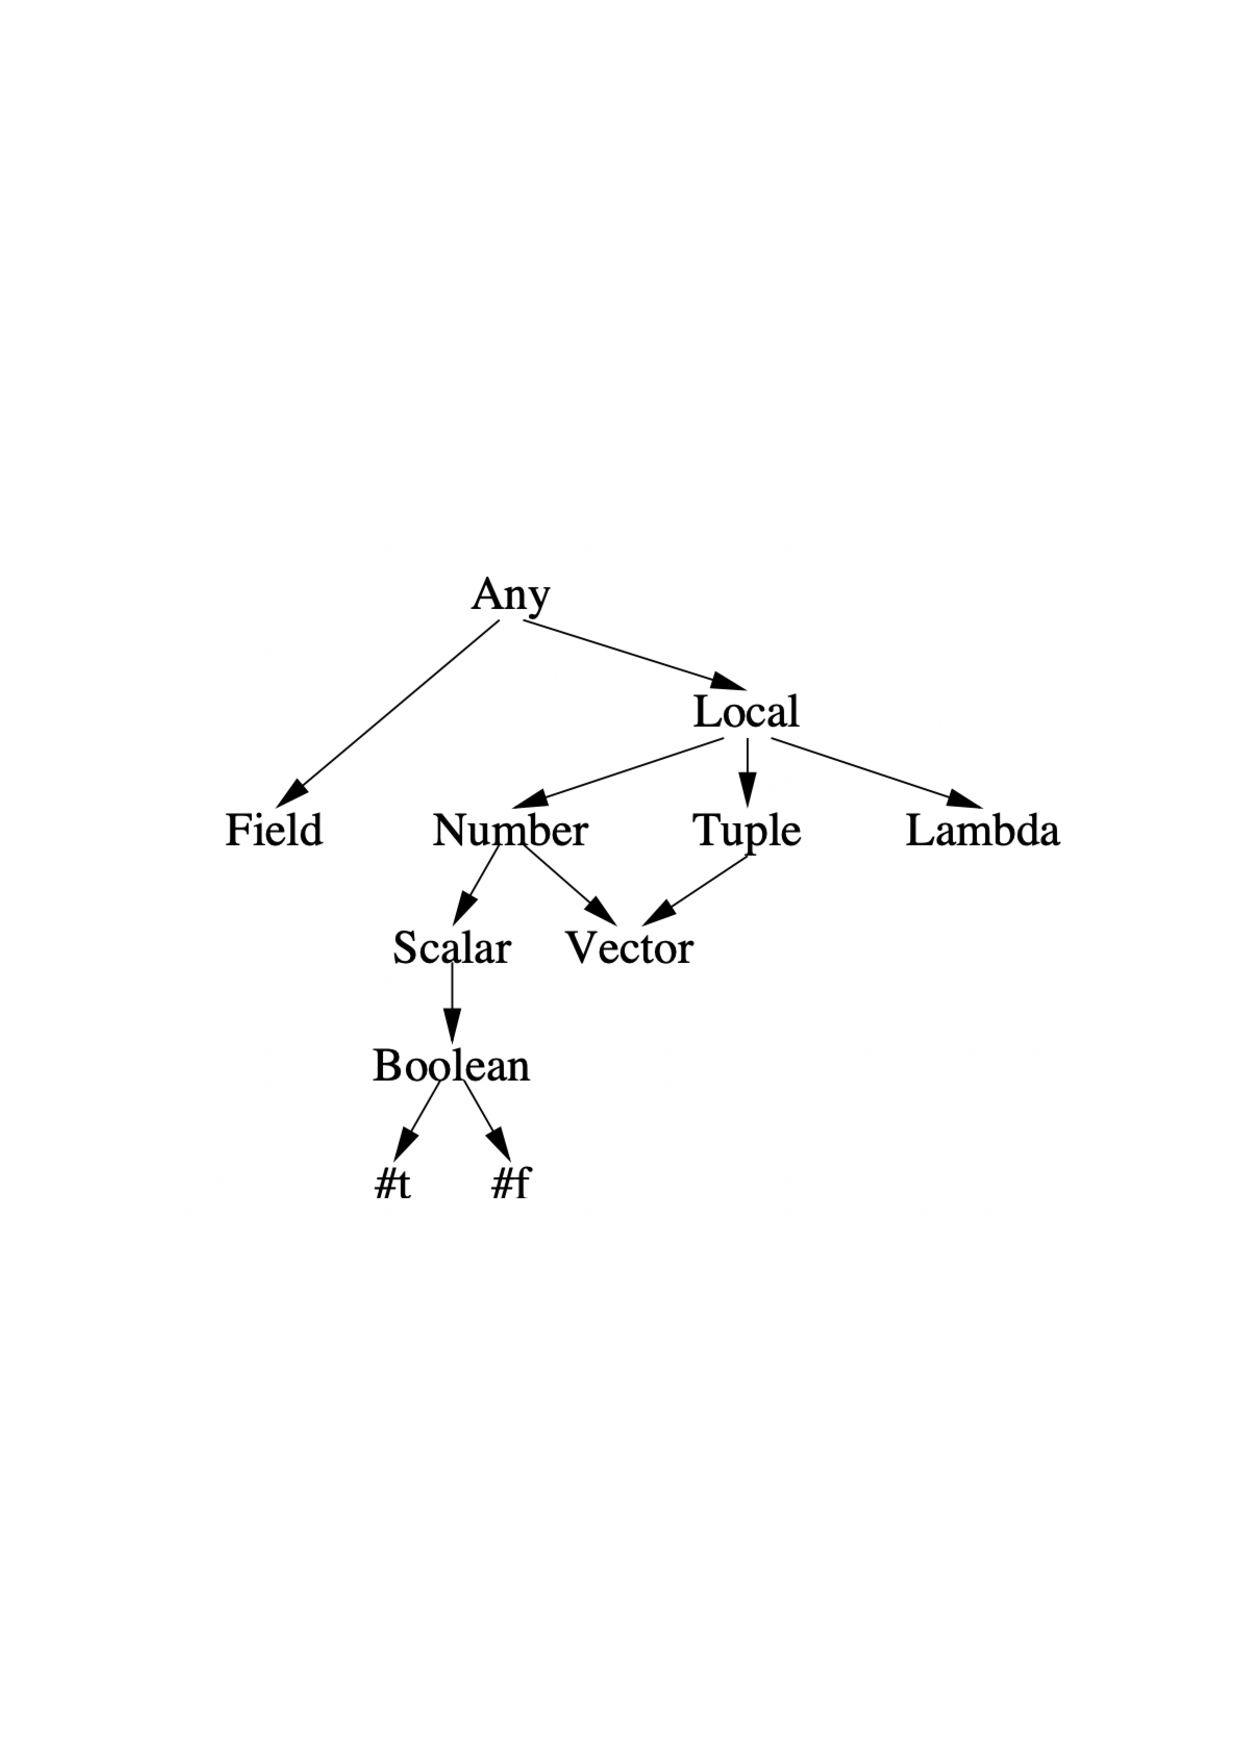
\includegraphics[width=.6\linewidth]{figures/type-system-proto.pdf}
    \caption{Gerarchia dei tipi di dato in Proto.}
    \label{fig:mitproto-types}
\end{figure}

\begin{itemize}
    \item \texttt{Any}: Radice della gerarchia dei tipi.
    \item \texttt{Field}: Rappresenta un campo di vicinato \(\phi\), associando a ogni dispositivo un valore locale (\texttt{Local}). 
    \item \texttt{Local}: Rappresenta qualsiasi valore che non sia un \texttt{Field}. I sottotipi di \texttt{Local} includono:
    \begin{itemize}
        \item \texttt{Tuple}: Insieme ordinato di valori locali (\texttt{Local}).
        \item \texttt{Scalar}: Numero a virgola mobile, inclusi i valori speciali \texttt{nan}, \texttt{inf} e \texttt{-inf}.
        \item \texttt{Vector}: Tupla (\texttt{Tuple}) di valori scalari (\texttt{Scalar}).
        \item \texttt{Number}: Valore scalare (\texttt{Scalar}) o vettoriale (\texttt{Vector}).
        \item \texttt{Boolean}: Valore booleano true (\texttt{\#t}) o false (\texttt{\#f}).
        \item \texttt{Lambda}: Funzione anonima.
    \end{itemize}
\end{itemize}

Nel seguito, i tipi di dato saranno indicati con la prima lettera maiuscola: ad esempio, una variabile \texttt{x} di tipo \texttt{Local} sarà denotata come \texttt{x|L}, mentre \texttt{y} di tipo \texttt{Field} come \texttt{y|F}.

\paragraph{Dichiarazione di funzioni e variabili} Le funzioni vengono dichiarate utilizzando la forma \texttt{(def \(nome\) (\(parametri\)) (\(corpo\)))}, dove \texttt{\(nome\)} è il nome della funzione, \texttt{\(parametri\)} è una lista di parametri formali e \texttt{\(corpo\)} è l'espressione che definisce il comportamento della funzione. Il tipo di ritorno della funzione è dedotto automaticamente in base al tipo dell'espressione \texttt{\(corpo\)}.

Le variabili vengono dichiarate tramite la parola chiave \texttt{let}, seguendo la sintassi \texttt{(let (\(nome\) (\(valore\))))}, dove \texttt{\(nome\)} è il nome della variabile, \texttt{\(valore\)} è l'espressione che ne determina il valore.

Se si desidera dichiarare più variabili contemporaneamente, si possono racchiudere più coppie \texttt{(\(nome\) (\(valore\)))} dentro il corpo di \texttt{let}. Se per definire le variabili successive si fa riferimento a quelle precedentemente dichiarate, dando importanza all'ordine di dichiarazione, si utilizza la parola chiave \texttt{let*}.

\section{Operatori}
\label{sec:mitprotooperators}

Proto fornisce un insieme di operatori che corrispondono ai costrutti fondamentali del field calculus (\cref{sec:fieldcalculus}).

\paragraph{Dinamica temporale} Per modellare lo stato di un dispositivo si sfrutta l'operatore \texttt{rep}, che segue la sintassi:

\lstinputlisting[
    language=Lisp,
    label={lst:mitprotoresp},
    caption={Sintassi dell'operatore \texttt{rep} in Proto.}
]{listings/proto/rep.proto}

\begin{itemize}
    \item \texttt{.var} è il nome della variabile di stato locale.
    \item \texttt{init} è l'espressione che inizializza il valore della variabile di stato.
    \item \texttt{evolve} è l'espressione che definisce come il valore della variabile di stato evolve nel tempo.
    \item Il tipo di ritorno dell'operatore è lo stesso tipo dell'espressione \texttt{init} ed \texttt{evolve}.
\end{itemize} 
L'esempio in \cref{lst:mitprotoresp} illustra l'uso di \texttt{rep} per creare un contatore che incrementa il proprio valore ad ogni round di esecuzione. 

\paragraph{Interazione Spaziale} L'operatore \texttt{nbr} consente a un dispositivo di accedere ai valori calcolati dai vicini nell'ultimo round di esecuzione. La sintassi è la seguente:

\lstinputlisting[
    language=Lisp,
    label={lst:mitprotonbr},
    caption={Sintassi dell'operatore \texttt{nbr} in Proto.}
]{listings/proto/nbr.proto}

\begin{itemize}
    \item \texttt{expr} è l'espressione il cui valore locale viene raccolto dai vicini.
    \item Il tipo di ritorno dell'operatore è un \texttt{Field} che mappa l'identificatore di ogni vicino al valore locale risultante dalla valutazione di \texttt{expr} in quel dispositivo.
\end{itemize}

In \cref{lst:mitprotonbr} viene mostrato un esempio di utilizzo di \texttt{nbr} nel quale si costruice un campo di vicinato che associa \(1\) ad ogni vicino.

Proto fornisce varianti dell'operatore \texttt{nbr} che permettono di raccogliere specifici valori dai vicini come \texttt{nbr-range}, per ottenere la distanza fisica tra il dispositivo corrente e ciascun vicino, e \texttt{nbr-vec}, per ottenere un vettore che indica la direzione verso ciascun vicino rispetto al dispositivo corrente.

Vengono fornite delle funzioni di aggregazione che permettono di ridurre un \texttt{Field} a un singolo valore locale (\texttt{Local}) (\Cref{lst:mitprotonbragg}).

\lstinputlisting[
    language=Lisp,
    label={lst:mitprotonbragg},
    caption={Esempi di funzioni di aggregazione spaziale in Proto.}
]{listings/proto/summary-functions.proto}

Queste funzioni si basano su \texttt{fold-hood} (\Cref{lst:mitprotofoldhood}), un operatore più generale che consente di specificare una funzione di combinazione personalizzata.

\lstinputlisting[
    language=Lisp,
    label={lst:mitprotofoldhood},
    caption={Sintassi dell'operatore \texttt{fold-hood} in Proto.}
]{listings/proto/fold.proto}

Si noti che \texttt{fold-hood} non richiede in ingresso un \texttt{Field}, bensì \texttt{value} è un valore locale (\texttt{Local}). Internamente, \texttt{fold-hood} utilizza l'operatore \texttt{nbr} per raccogliere i valori dai vicini in modo trasparente al programmatore e applica la funzione di combinazione specificata per aggregarli.

\paragraph{Restrizione dello spazio} L'operatore \texttt{if} partiziona lo spazio dei dispositivi in due sottoinsiemi in base alla valutazione di una condizione. La sintassi è la seguente (\Cref{lst:mitprotoif}):

\lstinputlisting[
    language=Lisp,
    label={lst:mitprotoif},
    caption={Sintassi dell'operatore \texttt{if} in Proto.}
]{listings/proto/if.proto}

\begin{itemize}
    \item \texttt{test} è l'espressione booleana che determina la partizione dello spazio.
    \item \texttt{true} è l'espressione che viene valutata nei dispositivi per cui \texttt{test} è vera.
    \item \texttt{false} è l'espressione che viene valutata nei dispositivi per cui \texttt{test} è falsa.
    \item Il tipo di ritorno dell'operatore è lo stesso di \texttt{true} e \texttt{false}.
\end{itemize}

Anche se \texttt{true} e \texttt{false} dovessero risultare la stessa espressione, il loro valore potrebbe differire, in accordo a quanto detto in \cref{sec:fieldcalculus}.

È possibile utilizzare l'operatore \texttt{mux} come alternativa a \texttt{if} quando si desidera che le due espressioni \texttt{true} e \texttt{false} vengano valutate prima del partizionamento, garantendo la partecipazione di tutti i dispositivi alla computazione (\Cref{sec:fieldcalculus}).

\section{Funzioni di libreria}
\label{sec:mitprotobuiltin}

Proto è equipaggiato con una libreria che fornisce diverse funzioni comuni durante lo sviluppo di programmi aggregati. 

\begin{itemize}
    \item \texttt{(distance-to ,source|B) -> S}: calcola la distanza minima dalla sorgente per ogni dispositivo. I nodi in cui \texttt{source} è \texttt{\#t} fungono da origine, mentre gli altri ricevono la distanza dalla sorgente più vicina. \texttt{gradient} è un alias di questa funzione.
    \item \texttt{(broadcast ,source|B ,value|L) -> L}: propaga il valore locale \texttt{value} dai dispositivi sorgente verso l'intera rete. Ogni dispositivo riceve il valore dalla sorgente più vicina.
    \item \texttt{(dilate ,source|B ,d|S) -> B}: Verifica quali dispositivi si trovano entro una distanza \texttt{d} dalla sorgente più vicina.
    \item \texttt{(distance ,r1|B ,r2|B) -> S}: calcola la distanza tra le due regioni \texttt{r1} e \texttt{r2} e la propaga in tutta la rete.
    \item \texttt{(timer) -> S}: restituisce il tempo trascorso durante la valutazione dell'espressione nel dispositivo corrente.
\end{itemize}

Inoltre sono fornite funzioni per operare con i tipi di dato elencati in \cref{fig:mitproto-types}, come operazioni aritmetiche, logiche, di confronto, manipolazione di tuple e di vettori, nonché funzioni per la generazione di numeri casuali.

\lstinputlisting[
    language=Lisp,
    label={lst:mitprotobuiltin},
    caption={Funzioni di built-in in Proto.}
]{listings/proto/utilities.proto}

Nel simulatore di Proto, ciascun nodo è dotato di sensori e sonde per interagire con l'ambiente. Le istruzioni \texttt{sense} e \texttt{probe} permettono rispettivamente la lettura dai sensori e la scrittura sulle sonde. In particolare, \texttt{(probe (e1) idx)} invia il valore di \texttt{e1} alla sonda \texttt{idx} e lo restituisce come risultato.

